%%==================================================================%%
%% Author : P�rez Ruiz, Alejandro                                   %%
%% Author : S�nchez Barreiro, Pablo                                 %%
%% Version: 1.1, 14/06/2011                                         %%
%%                                                                  %%
%% Memoria del Proyecto Fin de Carrera                              %%
%% Cap�tulo Domain Engineering, Archivo ra�z                        %%
%%==================================================================%%

\chapterheader{Ingenier�a del Dominio}{Ingenier�a del Dominio}
\label{chap:domain}

Este cap�tulo se describe la fase de \emph{ingenier�a del dominio} (en ingl�s, \emph{Domain Engineering}) de nuestra l�nea de productos software. Dentro de dicha fase, se detalla la definici�n de la arquitectura de la familia de productos y se detallan las iteraciones m�s relevantes de este proceso de desarrollo. Las otras iteraciones, por motivos de espacio y con objeto de no aburrir al lector con detalles irrelevantes, simplemente se omiten.

\chaptertoc

\section{Definici�n Arquitect�nica}

%%==================================================================%%
%% Author : P�rez Ruiz, Alejandro                                   %%
%% Author : S�nchez Barreiro, Pablo                                 %%
%% Version: 1.1, 16/01/2011                                         %%                                                                                    %%                                                                  %%
%% Memoria del Proyecto Fin de Carrera                              %%
%% Domain Engineering/Architecture                                  %%
%%==================================================================%%

Un hogar inteligente posee una serie de dispositivos que se descomponen en \emph{sensores} y \emph{actuadores}. Los \emph{sensores} son los encargados de obtener los datos del elemento al que pertenecen, como por ejemplo, los grados que hace en una habitaci�n, la apertura que tiene una ventana... Los \emph{actuadores} se encargan de ejecutar las ordenes, por ejemplo que una persiana se abra o se cierre, la calefacci�n se encienda a unos determinados grados...

Tanto los sensores como los actuadores se encuentran conectados a un dispositivo central que los coordina, el cual se conoce como \emph{puerta de enlace} (en ingl�s, \emph{Gateway}). Dicho Gateway se encarga de leer los datos de los sensores, procesarlos y enviar las ordenes adecuadas a los actuadores. De igual modo, el Gateway recibe ordenes de los usuarios que son ejecutadas por los actuadores para modificar los elementos de la casa.

%%=====================================================================%%
%% HECHO(Pablo): Aqu� hace falta una figura describiendo la            %%
%%              arquitectura                                           %%
%% http://www.google.es/imgres?imgurl=http://www.fancybread.com/blog/images//mediator.jpg&imgrefurl=http://www.fancybread.com/blog/post.cfm/mediator-pattern-applied-to-javascript&h=273&w=316&sz=25&tbnid=x1f5CI5WvMYNzM:&tbnh=101&tbnw=117&prev=/search%3Fq%3DMediator%2BPattern%26tbm%3Disch%26tbo%3Du&zoom=1&q=Mediator+Pattern&hl=es&usg=__ZG2xo8qDKX8sPv-uWS_mDcE-zQo=&sa=X&ei=MnL7TZLvNcWYhQfkrYizAw&ved=0CEcQ9QEwBQ
%%=====================================================================%%
Por tanto, tal como se ve en la Figura~\ref{domain:fig:mediator}, el dise�o de nuestra arquitectura es una aplicaci�n concreta del patr�n de dise�o \emph{mediador}~\cite{gamma:1994}, donde el \emph{Gateway} ejercer el papel de mediador, y los diferentes sensores y actuadores son los distintos elementos a coordinar. El objetivo de este patr�n es extraer y encapsular en una �nica clase la l�gica de coordinaci�n de un conjunto de objetos que necesitan interaccionar entre ellos siguiendo reglas de coordinaci�n de cierta complejidad. Al encapsular esta l�gica en un �nico objeto, denominado \emph{mediador} , el dise�o de los diferentes objetos que deben interactuar, en nuestro caso sensores y actuadores,  se simplifica, ya que estos elementos ahora s�lo tienen que notificar eventos al mediador y recibir notificaciones del mismo. Del mismo modo, cualquier cambio en la l�gica de coordinaci�n de estos objetos afecta solo a la clase \emph{Mediador}, el \emph{Gateway} en nuestro caso, en lugar de a los diferentes objetos que toman parte en la interacci�n.
\begin{figure}[!h]
 \centering
 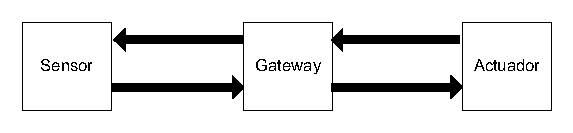
\includegraphics[width=.55\linewidth]{domainEngineering/images/Mediator.eps} \\
 \caption{Dise�o de la arquitectura a trav�s del patr�n de dise�o \emph{mediador}}
 \label{domain:fig:mediator}
\end{figure}

Adem�s de los sensores y actuadores, para que el usuario pueda controlar y visualizar el estado de los diversos dispositivos es necesario la creaci�n de una interfaz gr�fica que permita al usuario interactuar con el \emph{Gateway}.

Esta interfaz gr�fica tendr� que actualizar el estado de sus elementos cuando se producen cambios en los dispositivos. Para simplificar esta dependencia entre la interfaz gr�fica y el \emph{Gateway}, haremos uso del patr�n \emph{Observador}~\cite{gamma:1994} (\emph{Observer pattern}, en ingl�s). Para instanciar este patr�n, el \emph{Gateway} contendr� una lista por cada dispositivo que pueda ser observado. Los objetos interesados en ser notificados cada vez que dicho dispositivo cambie su estado se registrar�n o a�adir�n en dicha lista. De esta forma, cada vez que un dispositivo cambia de estado, el \emph{Gateway} notifica dicho cambio a todos los objetos registrados en la correspondiente lista de \emph{observadores}.

Finalmente, y dado que este proyecto no trabaja con actuadores y sensores reales, es necesario simular mediante software dichos dispositivos. Por ejemplo, deberemos simular variables tales como la temperatura percibida por los sensores, o el transcurso del tiempo del sistema. Para ello crearemos una interfaz gr�fica que juegue el papel de simulador, y permita al usuario interactuar con los dispositivos a simular as� como alterar diversas variables externas al sistema, como la temperatura.

Una vez definido el dise�o arquitect�nico b�sico, se desarrollan las iteraciones necesarias para completar la fase de ingenier�a del dominio. La siguiente secci�n describe los principios de dise�o seguidos para la construcci�n de dichas caracter�sticas. 

\section{Principios de Dise�o}
\label{domain:sec:pattern}

%%==================================================================%%
%% Author : P�rez Ruiz, Alejandro                                   %%
%% Author : S�nchez Barreiro, Pablo                                 %%
%% Version: 1.1, 14/06/2011                                         %%
%%                                                                  %%
%% Memoria del Proyecto Fin de Carrera                              %%
%% Domain Engineering/Interacion Dos                                %%
%%==================================================================%%

Para dise�ar nuestra l�nea de productos software seguimos un enfoque similar al de CaesarJ (cf.~\ref{back:subsec:foLanguages}), tratando de encapsular cada caracter�stica en una familia de clases.
La Figura~\ref{domain:fig:packageDiagram} muestra la descomposici�n en caracter�sticas de nuestro problema, as� como las dependencias entre las diferentes caracter�sticas. Siguiendo los principios de dise�o propuestos dentro del proyecto AMPLE~\cite{ample:d22}, cada familia de clases se representa como un paquete UML y las relaciones de herencia entre familias de clases como relaciones \emph{merge} entre paquetes.

\begin{figure}[!h]
 \centering
 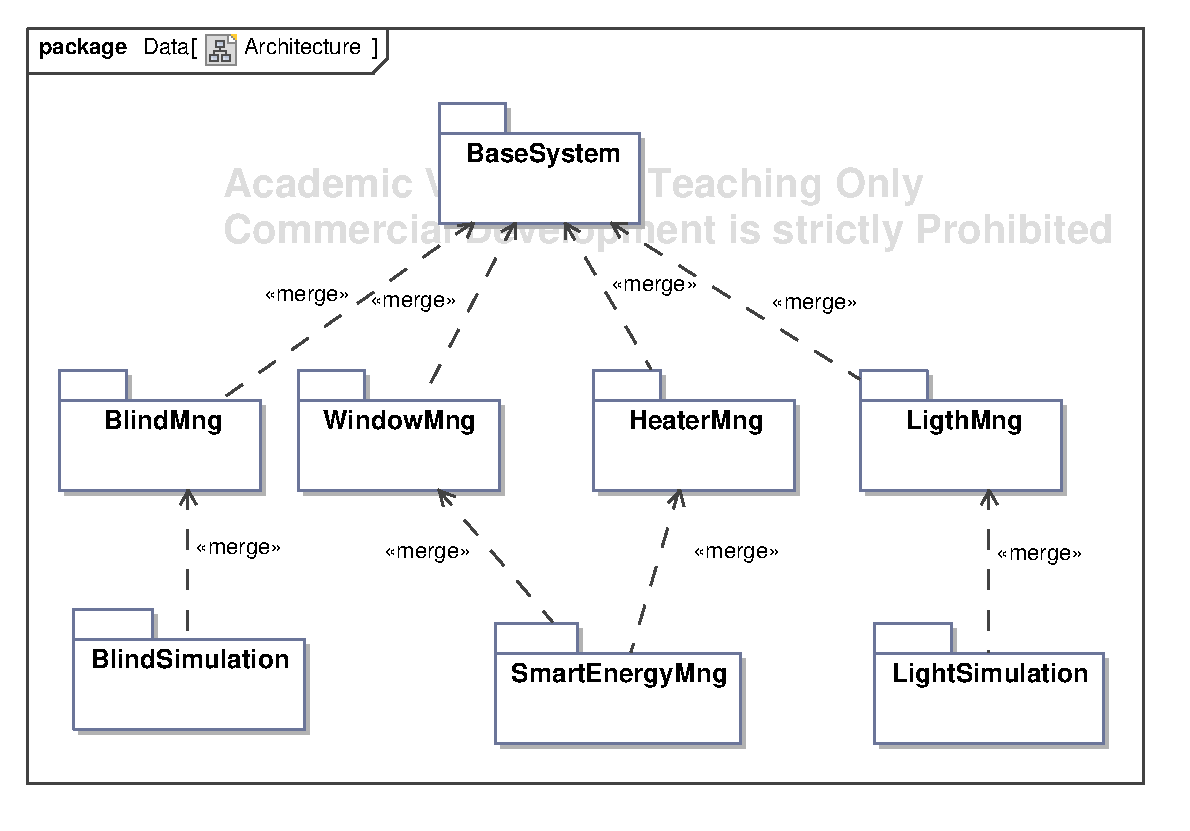
\includegraphics[width=.55\linewidth]{domainEngineering/images/packageDiagram.eps} \\
 \caption{Descomposici�n Orientada a Caracter�sticas de nuestra LPS}
 \label{domain:fig:packageDiagram}
\end{figure}

Para simular los mecanismos proporcionados por CaesarJ, usaremos las clases parciales de C\#. De esta forma, cada clase contenida en uno de los paquetes de la Figura~\ref{domain:fig:packageDiagram} se implementar� como una clase parcial que pueda ser extendida con nuevas funcionalidades en subsiguientes caracter�sticas. No obstante, el principal problema de este esquema es que las clases parciales, tal como ha sido identificado por~\cite{elio:2010},
no permiten la sobreescritura de m�todos. Este problema aparece cuando se da una situaci�n como la de la  Figura~\ref{domain:fig:override}.

%%====================================================================%%
%% HECHO(Pablo): Ajusta los tama�os para que quede bonito              %%
%%====================================================================%%
\begin{figure}[!h]
 \centering
 \includegraphics[width=.40\linewidth]{domainEngineering/images/overriding.eps} \\
 \caption{Problema de la sobreescritura con m�todos parciales C\#}
 \label{domain:fig:override}
\end{figure}

En este caso, la clase \imp{A} de la caracter�stica \imp{FeatureY} debe sobreescribir el m�todo \imp{aMethod()} de la versi�n de la clase \imp{A} para la caracter�stica \imp{FeatureX} con objeto de alterar su funcionalidad. Si la clase \imp{A} est� implementada como clase parcial de C\# en las caracter�sticas \imp{FeatureX} y \imp{FeatureY}, al intentar combinarlas el compilador reportar� un error indicando que existen m�todos con id�ntico perfil en clases parciales distintas. Este error se produce porque el compilador no soporta la fusi�n de m�todos o \emph{m�todos parciales}, lo cual es bastante l�gico. Dados dos m�todos con id�ntica cabecera, pero con implementaciones distintas, lo extra�o ser�a que el compilador supiese como fusionar dichas implementaciones de forma correcta.

Por tanto, hemos de idear un m�todo para poder sobreescribir m�todos. La soluci�n planteada se ilustra en la Figura~\ref{domain:fig:overrideSolution}. Dado que no podemos tener m�todos con id�ntico nombre y argumentos en diferentes clases parciales, cada m�todo correspondiente a una caracter�stica se precede con el nombre de la caracter�stica a la cual pertenece. Teniendo en cuenta que cada clase parcial pertenece a una caracter�stica diferente, si cada caracter�stica tiene un nombre �nico, nos aseguraremos de que no existir� colisi�n entre nombres de m�todos.

Cuando queremos crear un producto espec�fico, seguiremos la siguiente estrategia. Crearemos una nueva familia de clases que represente el producto final (\imp{aProduct}). Dicha familia de clases contendr� una clase parcial por cada clase distinta contenida en una caracter�stica seleccionada. Las clases contenidas en la familia de clases representando el producto espec�fico contendr�n un m�todo por cada m�todo distinto (sin considerar el prefijo del nombre que indica la caracter�stica a la cual pertenece). Por �ltimo, cada m�todo delegar� en la versi�n correspondiente a la versi�n m�s profunda de dicho m�todo en el �rbol de herencia entre familias de clases.

%%====================================================================%%
%% HECHO(Pablo): Ajusta los tama�os para que quede bonito              %%
%%====================================================================%%
\begin{figure}[!h]
 \centering
 \includegraphics[width=.40\linewidth]{domainEngineering/images/solution.eps} \\
 \caption{Soluci�n para el problema de la sobreescritura}
 \label{domain:fig:overrideSolution}
\end{figure}

Ilustramos dicha soluci�n con un ejemplo concreto, el cual se ilustra en la Figura~\ref{domain:fig:overrideSolution}. En dicha soluci�n, s�lo la caracter�stica \imp{FeatureX} debe incluirse dentro del producto concreto a construir. Tal como indica nuestro patr�n de soluci�n, creamos una familia de clases \imp{aProduct} para representar el producto concreto deseado. A continuaci�n, a�adimos la clase parcial \imp{A} a dicha familia de clases, por estar dentro de la caracter�stica \imp{FeatureX}. Seguidamente, a�adimos el m�todo \imp{aMethod} a la recientemente creada clase \imp{A}. Este m�todo delegar� en la operaci�n \imp{featureX\_aMethod}, por ser la versi�n correspondiente a este m�todo perteneciente a una caracter�stica seleccionada y que se encuentra m�s profunda en el �rbol de herencia entre familias de clases.

En las siguientes secciones describimos como siguiendo los principios de dise�o expuestos en esta secci�n, se han creado las iteraciones necesarias para crear el sistema base, controlar aparatos de fr�o/calor, las ventanas y el control inteligente de energ�a. Se han elegido estas interacciones, y no otras, por parecernos las m�s interesantes. Las otras se omiten por ser similares a �stas y por motivo de espacio.


\section{Iteraci�n 1: Sistema Base}

%%==================================================================%%
%% Author : P�rez Ruiz, Alejandro                                   %%
%% Author : S�nchez Barreiro, Pablo                                 %%
%% Version: 1.1, 14/06/2011                                         %%
%%                                                                  %%
%% Memoria del Proyecto Fin de Carrera                              %%
%% Domain Engineering/BaseSystem                                    %%
%%==================================================================%%

En la primera iteraci�n debemos definir la estructura b�sica del patr�n \emph{Mediador}. Adem�s, deberemos crear el esquema b�sico de la interfaz gr�fica, la cual deber� permitir controlar hogares con un n�mero de plantas y habitaciones variable. Adem�s la interfaz gr�fica deber� permitir la incorporaci�n de nuevas subinterfaces para el control de diversas funcionalidades, como por ejemplo, el control autom�tico de luces o ventanas. Los requisitos concretos que se han de satisfacer en esta iteraci�n se muestran en la Figura~\ref{plan:table:requisitos}.

%%====================================================================%%
%% NOTA(Pablo): Haz esta imagen m�s ancha que larga, m�s compacta y   %%
%%              m�s sim�trica                                         %%
%%====================================================================%%

\begin{figure}[!tb]
 \centering
 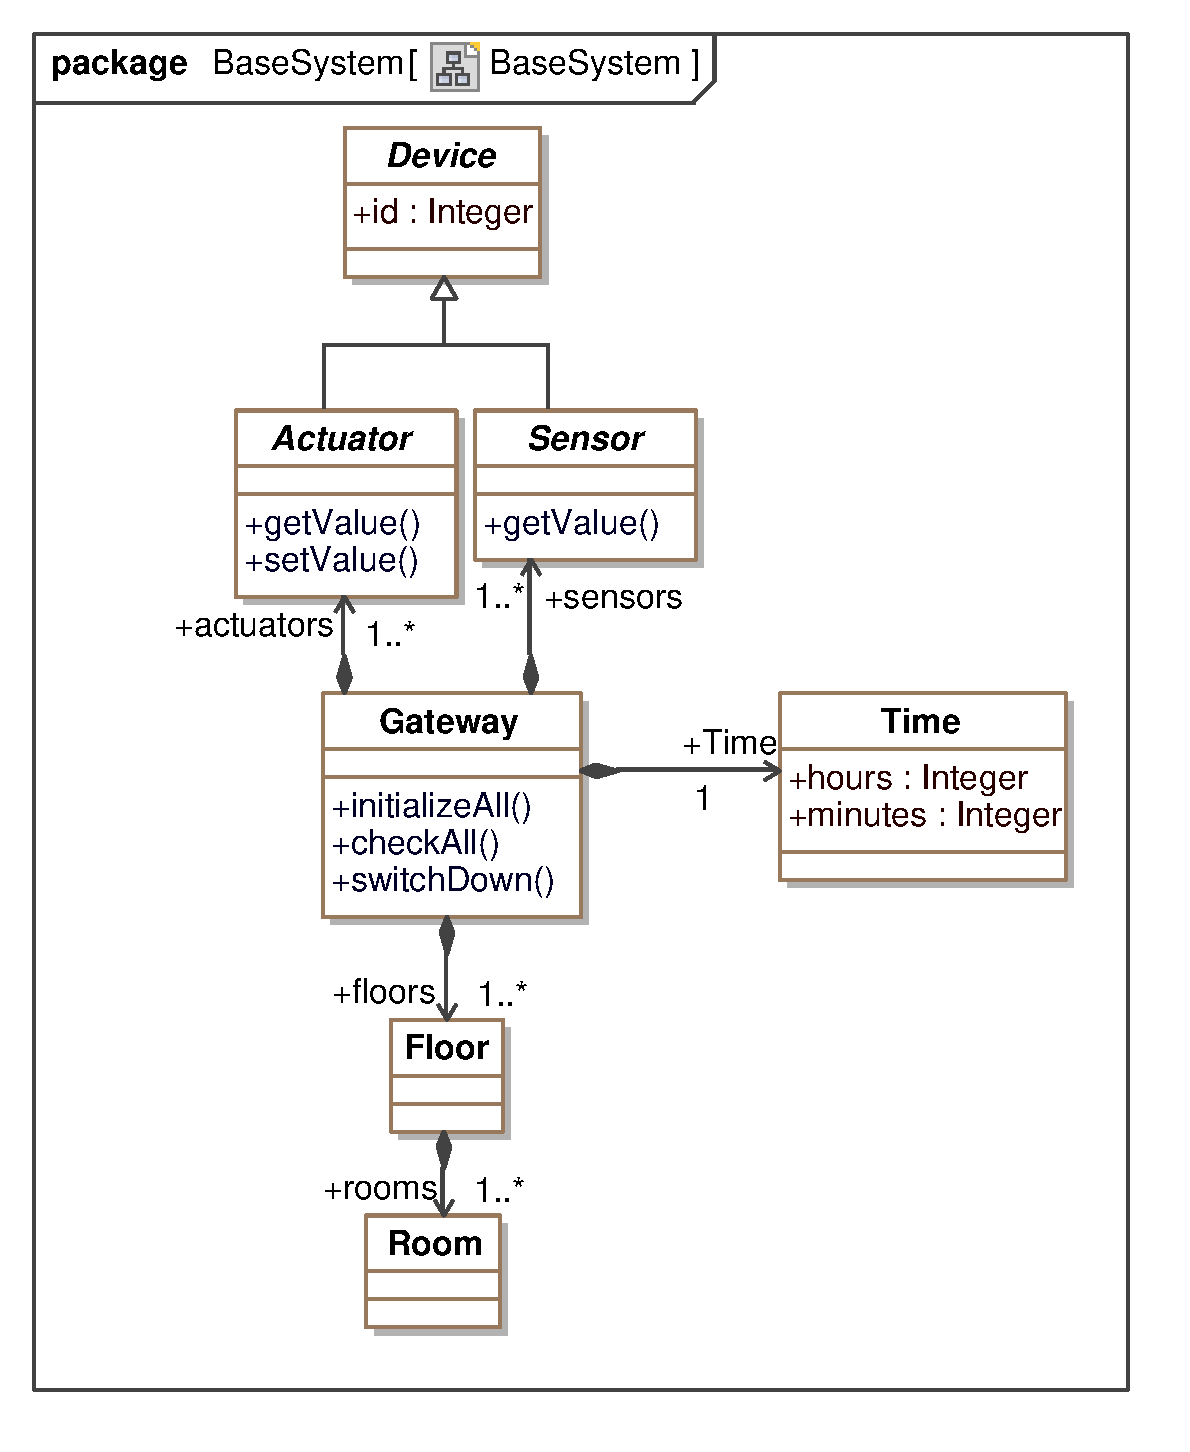
\includegraphics[width=.45\linewidth]{domainEngineering/Images/definicionArq.eps} \\
 \caption{Dise�o del sistema base}
 \label{domain:fig:defArq}
\end{figure}


La Figura~\ref{domain:fig:defArq} muestra el dise�o realizado para esta caracter�stica. Tal como se observa, el \emph{Gateway} posee una lista de plantas y a su vez cada planta contiene otra lista de las habitaciones que se encuentran en dicha planta. Se crea adem�s un objeto tiempo que se encarga de simular el transcurso del tiempo en el sistema. Todas las clases de la Figura~\ref{domain:fig:defArq} se implementar�n como clases parciales de C\#, de forma que puedan ser extendidas con nuevas funcionalidades en subsiguientes caracter�sticas.

%%====================================================================%%
%% NOTA(Pablo): Esto es redundante                                    %%
%%====================================================================%%
%%
%% Una parte importante del sistema son las interfaces gr�ficas que 
%% permitir�n al usuario interactuar con el Gateway. Se implementan 
%% dos, la primera de ellas permite al usuario actuar con el Gateway, 
%% mientras que la segunda har� el papel de simulador, ya que es 
%% necesario modificar algunos valores que deber�an ser alterados 
%% por elementos externos al propio sistema, tales como la temperatura 
%% actual de una habitaci�n o el tiempo,ya que el sistema no se 
%% encuentra conectado a dispositivos reales.
%%
%%====================================================================%%

A la par que la l�gica del sistema, debemos crear las interfaces gr�ficas que permitan al usuario interactuar con el sistema. No obstante, no debemos olvidar que estamos implementado una l�nea de productos software, por lo que todos los dise�os de las interfaces gr�ficas deben adaptarse a cualquier composici�n de caracter�sticas que haga un usuario.

\begin{figure}[!tb]
 \centering
 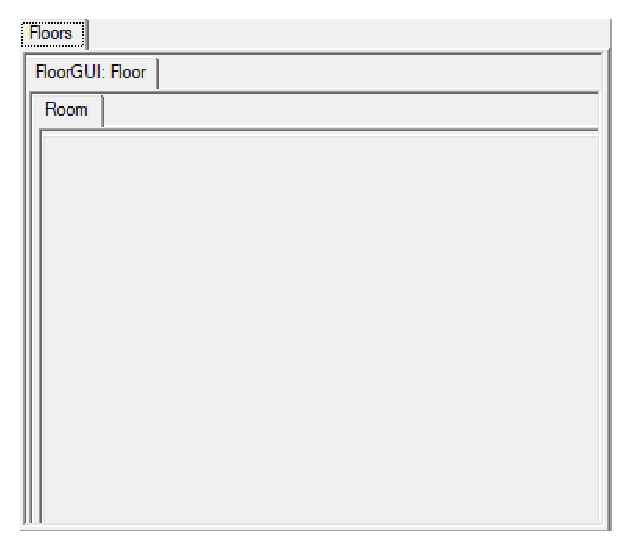
\includegraphics[width=.55\linewidth]{domainEngineering/Images/GUI.eps} \\
 \caption{Dise�o de la interfaz gr�fica de usuario}
 \label{domain:fig:gatewayGUI}
\end{figure}

Como punto de partida para el dise�o de las interfaces gr�ficas se ha utilizado la API para el desarrollo de aplicaciones gr�ficas que incluye .NET, denominada \emph{Windows Forms}~\cite{brown:2006}. Debido a que el n�mero de plantas y el
e habitaciones debe ser variable, la interfaz deber� permitir la visualizaci�n de una cantidad arbitraria de plantas. Adem�s, cuando una planta sea seleccionada se deber�n mostrar todas las habitaciones que contiene, y cada habitaci�n debe de poder contener diferentes caracter�sticas, tales como control de ventanas, persianas, luces, etc. Por todo lo citado anteriormente, se ha decidido utilizar un dise�o como el mostrado en la figura \ref{domain:fig:gatewayGUI}. En dicho dise�o, cada planta se representa como una pesta�a. Cada pesta�a que contiene habitaciones, representadas como pesta�as anidadas. A su vez, por cada caracter�stica seleccionada en una habitaci�n, se crear� una nueva pesta�a anidada, dentro de la pesta�a de cada habitaci�n.

%%====================================================================%%
%% NOTA(Pablo): Esto es demasuiado detalle irrelevante
%%====================================================================%%
%%
%% Con esta API para construir una interfaz gr�fica se deben a�adir 
%% controles a una forma e implementar respuestas a las acciones de los 
%% usuarios, tales como un click de rat�n o la pulsaci�n de una tecla. 
%% Un control se define como una interfaz de usuario que muestra datos 
%% o acepta datos de entrada. Por lo que lo primero que se debe pensar 
%% es en los controles que ser�n m�s adecuados para la ventana que 
%% contiene la interfaz gr�fica. 
%%
%%====================================================================%%

Siguiendo este mismo razonamiento, hemos creado el dise�o para la interfaz gr�fica del simulador. En el caso del sistema base, solo se encargar� de mostrar las plantas y habitaciones que se han creado, por lo que se vuelve a seleccionar un control que permita a�adir pesta�as tal y como se muestra en la figura \ref{domain:fig:simulatorGUI} y una tabla con el identificador de una habitaci�n, su nombre y la planta a la que pertenecen.

\begin{figure}[!tb]
 \centering
 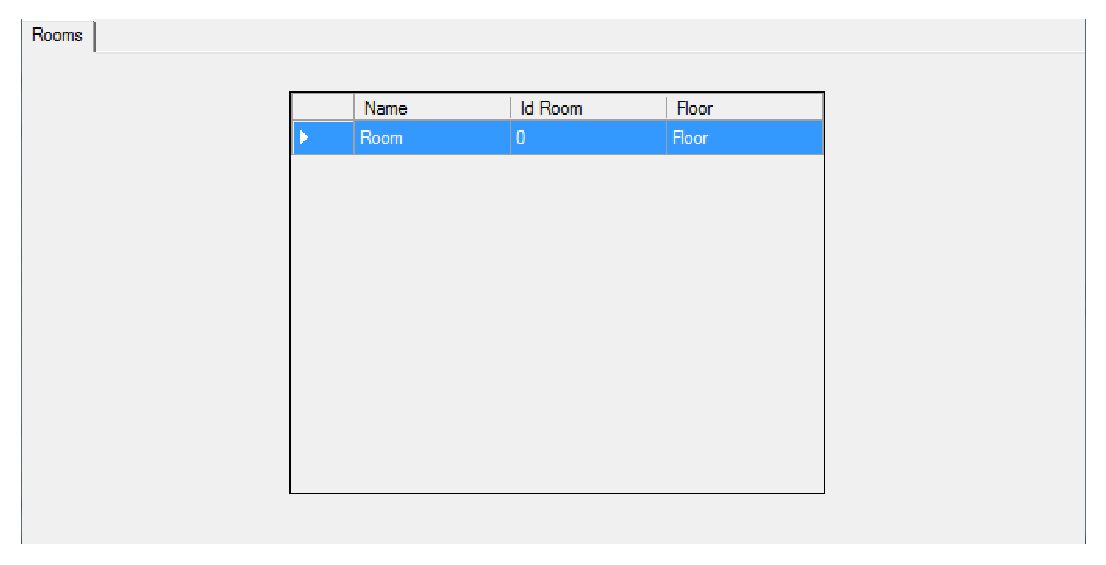
\includegraphics[width=.65\linewidth]{domainEngineering/Images/simulatorGUI.eps} \\
 \caption{Dise�o de la interfaz gr�fica para el simulador}
 \label{domain:fig:simulatorGUI}
\end{figure}

Para poder a�adir nuevas funcionalidades y caracter�sticas a ambas interfaces, �stas se implementan mediante clases parciales.

Una vez implementado todo el sistema base se realizaron una serie de test de prueba, cuyo objetivo era crear diferentes instancias del sistema para comprobar que tanto las plantas y habitaciones se creaban, a�ad�an y visualizaban en las interfaces gr�ficas correctamente.

Tras haber finalizado la implementaci�n del sistema base ya se tiene la infraestructura b�sica para poder crear nuevas caracter�sticas que extiendan y a�adan nuevas funcionalidades. La siguiente secci�n describe el proceso de desarrollo para la caracter�stica \emph{HeaterMng}, que se a�ade a este sistema base.


\section{Iteraci�n 2: Gesti�n de Sistemas de Control de Temperatura}

	%%==================================================================%%
	%% Author : P�rez Ruiz, Alejandro                                   %%
	%% Author : S�nchez Barreiro, Pablo                                 %%
	%% Version: 1.1, 14/06/2011                                         %%
	%%                                                                  %%
	%% Memoria del Proyecto Fin de Carrera                              %%
	%% Domain Engineering/Interacion Dos                                %%
	%%==================================================================%%

La caracter�stica de gesti�n de los sistemas de control de la temperatura  (\emph{HeaterMng}) deber�  permitir a los usuarios establecer el valor deseado para la temperatura (en grados Celsius). Los dispositivos de control de la temperatura funcionan como aparatos de fr�o/calor. De esta forma, si la temperatura especificada por el usuario es inferior a la actual, el dispositivo deber� enfriar la casa. En el caso opuesto, deber� calentarla.

%%=====================================================================%%
<<<<<<< .mine
%% NOTA(Pablo): Esto sobra
=======
%% NOTA(Pablo): Esto sobra                                          %%
>>>>>>> .r399
%%=====================================================================%%
%%
%% Para la situaci�n en la que la temperatura seleccionada por el
%% usuario coincida con la temperatura del lugar donde se encuentra el
%% calefactor, este �ltimo no entrar� en modo funcionamiento, por lo
%% que no consumir� energ�a.
%%
%%=====================================================================%%

Esta caracter�stica a�ade clases pare representar los nuevos dispositivos, m�s concretamente, \imp{Thermometer} y \imp{HeaterCtrl}, tal y como se ilustra en la Figura~\ref{domain:fig:heaterMngDesign}. Estos dispositivos extienden las clases abstractas \imp{Actuator} y \imp{Sensor}. Adem�s, se debe extender la clase \imp{Gateway} con nuevos m�todos y atributos para el control de estos nuevos dispositivos. A cada aparato de control de la temperatura se le asocia un term�metro en exclusiva, para realizar mediciones mas precisas.

\begin{figure}[!tb]
 \centering
 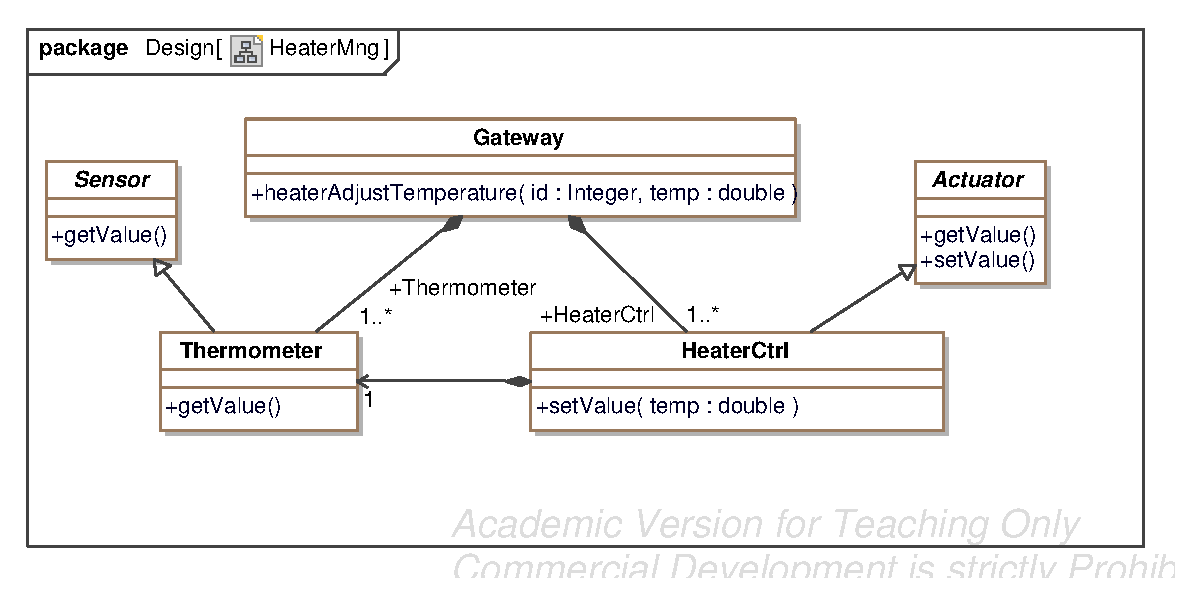
\includegraphics[width=.65\linewidth]{domainEngineering/Images/HeaterMngDesign.eps} \\
 \caption{Dise�o UML para la caracter�stica \emph{HeaterMng}}
 \label{domain:fig:heaterMngDesign}
\end{figure}

%%=====================================================================%%
%% NOTA(Pablo): Esto es trivial y no merece la pena contarlo
%%=====================================================================%%
%%
%% La principal acci�n que sostiene esta nueva caracter�stica es la de
%% modificar la temperatura de los calefactores por los usuarios del
%% sistema, por ello la figura \ref{domain:fig:secuenciaHeaterMng}
%% ilustra a trav�s de un diagrama de secuencia cuales son los pasos
%% de los mensajes necesarios para que la temperatura sea modificada.
%% Como ya se ha comentado en otras ocasiones en el diagrama de secuencia
%% se vuelve a observar como el Gateway es el mediador que se encarga de
%% transmitir los mensajes entre los distintos dispositivos.
%%
%%
%% \begin{figure}[!tb]
%5 \centering
%%  \includegraphics[width=.75\linewidth]
%%    {domainEngineering/Images/secuenciaHeaterMng.eps}%
%% \\
%% \caption{Diagrama de secuencia para modificar la temperatura.}
%%  \label{domain:fig:secuenciaHeaterMng}
%% \end{figure}
%%
%%=====================================================================%%

Tambi�n es necesario extender las dos interfaces gr�ficas que se implementaron en el sistema base. En el caso de la interfaz gr�fica para el control del \emph{Gateway}, a�adimos una nueva pesta�a a nivel global, para toda la casa, que permita encender o apagar todos los aparatos de control de la temperatura. En el caso de que los aparatos est�n conectados, se ofrecer� la opci�n de mostrar la temperatura deseada (ver Figura~\ref{domain:fig:GUIHeaterMng}). Pesta�as similares se a�aden a todas las plantas y habitaciones que contengan al menos un aparato de control de la temperatura.

%%=====================================================================%%
%% NOTA(Pablo): Con una captura vale. Aunque te haya costado trabajo,  %%
%%              esto no es del todo interesante. Deja la captura donde %%
%%              se ve todo                                             %%
%%=====================================================================%%

\begin{figure}[!tb]
 \centering
 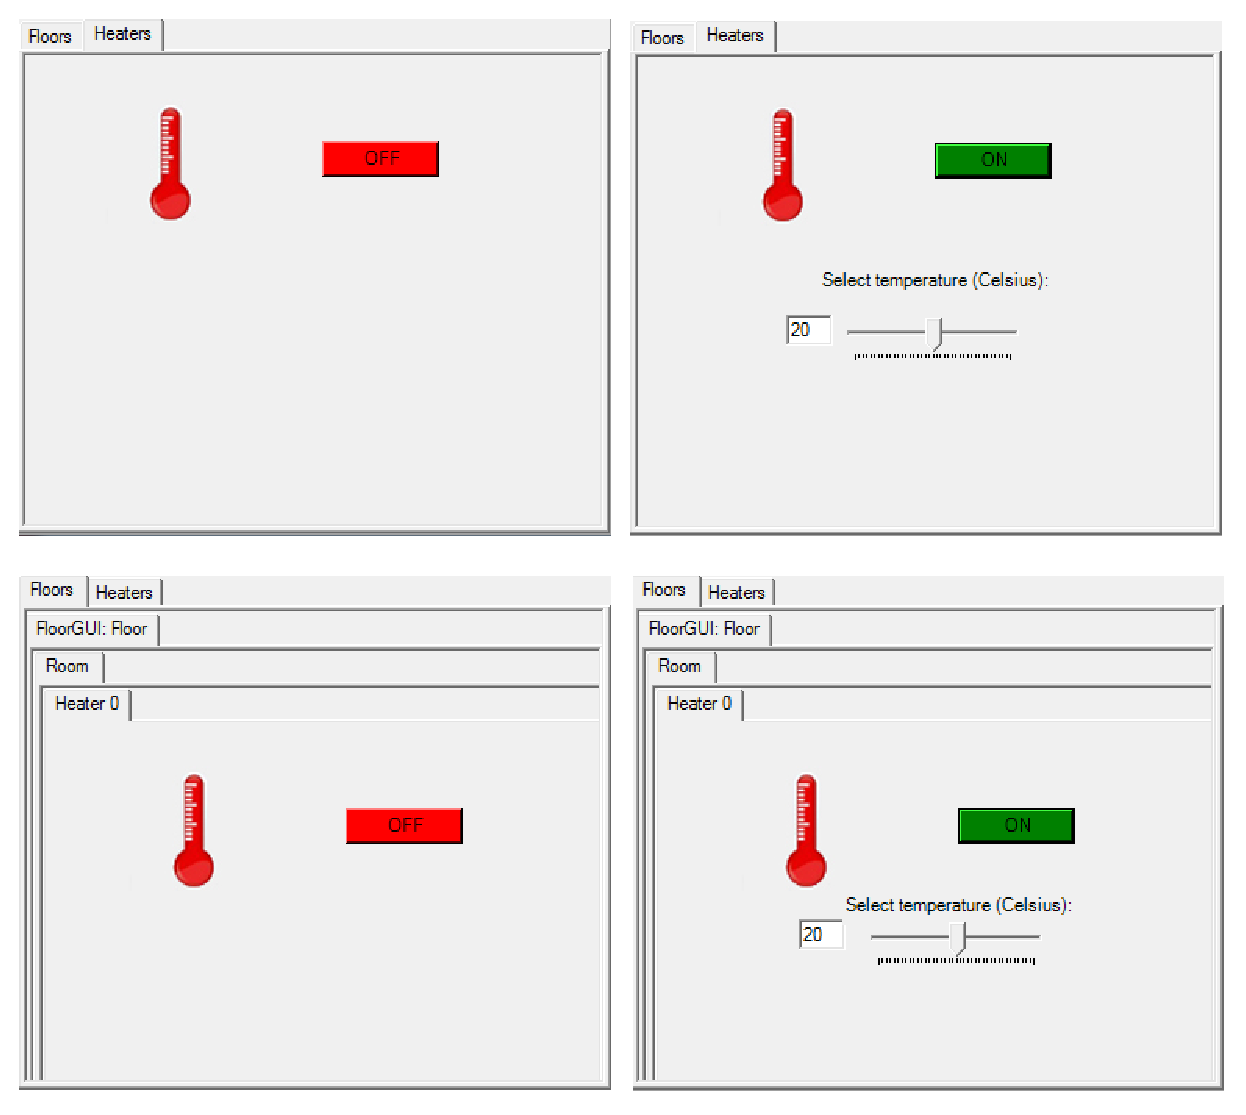
\includegraphics[width=.45\linewidth]{domainEngineering/Images/GUIHeaterMng.eps} \\
 \caption{Interfaz gr�fica de usuario con los elementos para el control de temperatura}
 \label{domain:fig:GUIHeaterMng}
\end{figure}

Por otro parte, tembi�n debemos extender la interfaz gr�fica del simulador. Por tanto, a�adimos una nueva pesta�a que muestre de forma tabular los diferentes aparatos de control de temperatura existentes en la casa as� como la informaci�n relacionada con los mismos de inter�s para observar el funcionamiento de la casa (ver Figura \ref{domain:fig:SimulatorHeaterMng}). Tambi�n se ofrece la posibilidad de cambiar el valor de la variable \emph{Temperatura} de cada term�metro, con objeto de analizar el comportamiento del hogar automatizado en diferentes situaciones.

\begin{figure}[!tb]
 \centering
 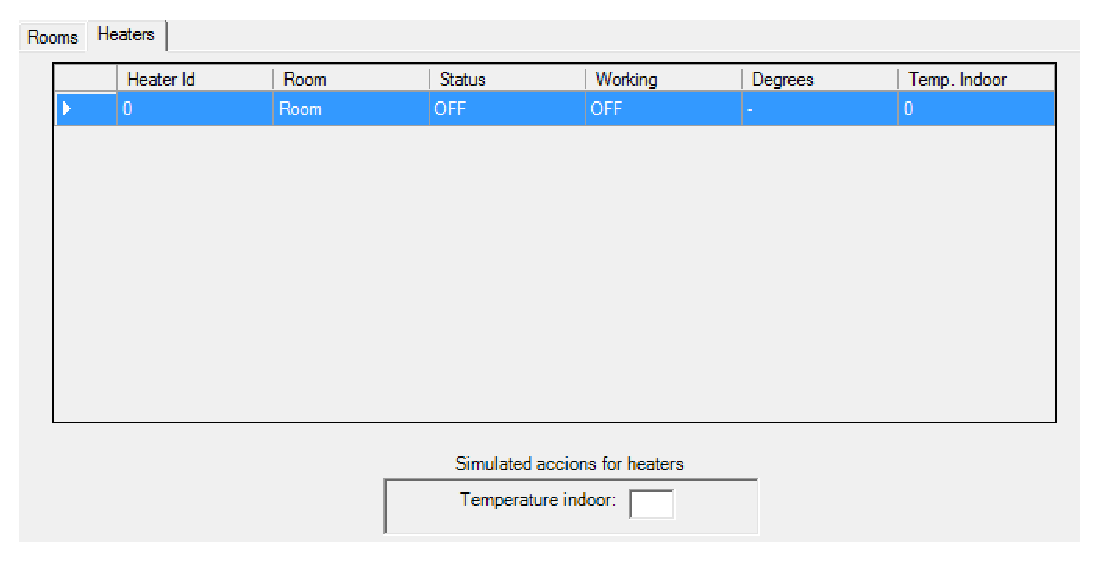
\includegraphics[width=.75\linewidth]{domainEngineering/Images/simulatorGUIHeaterMng.eps} \\
 \caption{Dise�o de la interfaz gr�fica de usuario para el simulador en la caracter�stica de \emph{HeaterMng}}
 \label{domain:fig:SimulatorHeaterMng}
\end{figure}

A continuaci�n, tanto el dise�o de la Figura~\ref{domain:fig:heaterMngDesign} como el de las interfaces mostradas en las Figuras~\ref{domain:fig:GUIHeaterMng} y~\ref{domain:fig:SimulatorHeaterMng}, se implementa usando los principios descritos en la Secci�n~\ref{domain:sec:pattern}. Por �ltimo, realizamos las pruebas de dicha implementaci�n. Los casos de prueba ejecutados se describen a continuaci�n:

\begin{enumerate}
\item Se han creado una serie de instancias del hogar inteligente con un n�mero de aparatos de control de la temperatura arbitrario y repartidos por distintas habitaciones.
\item Por cada instancia de un hogar concreto se ha verificado que se ejecutan correctamente las siguientes operaciones:
	\begin{enumerate}
		\item Es posible encender, apagar y modificar la temperatura de todos los aparatos de control de la temperatura a trav�s de la interfaz gr�fica de usuario. Dicho cambio se refleja adem�s en el simulador.
		%%=====================================================================%%
		%% NOTA(Pablo): Este caso de prueba no lo entiendo                     %%
		%%=====================================================================%%
		%% \item Por cada calefactor se modificar� su temperatura para que coincida con la de su term�metro, %% comprob�ndose que el calefactor cambie su modo de funcionamiento a sin consumo de energ�a.
		%%=====================================================================%%
		\item Es posible modificar la temperatura de los term�metros, y dicha alteraci�n afecta de forma correcta al modo de funcionamiento de los aparatos de control de la temperatura.
		\item Cuando el usuario modifica la temperatura deseada, los aparatos de fr�o/calor alteran su funcionamiento de la forma prevista.
	\end{enumerate}
\end{enumerate}




\section{Iteraci�n 3: Control Autom�tico de Ventanas}

%%==================================================================%%
%% Author : P�rez Ruiz, Alejandro                                   %%
%% Author : S�nchez Barreiro, Pablo                                 %%
%% Version: 1.1, 18/06/2011                                         %%
%%                                                                  %%
%% Memoria del Proyecto Fin de Carrera                              %%
%% Domain Engineering/Interacion Tres                               %%
%%==================================================================%%

La caracter�stica para en control autom�tico de ventanas tiene como principal requisito permitir a los usuarios abrir o cerrar una ventana con una determinada apertura (cf. Tabla~\ref{plan:table:requisitos}).

La Figura~\ref{domain:fig:designWindowMng} muestra el dise�o UML para esta caracter�stica, el cual se ha realizado siguiendo un proceso muy similar al de la secci�n anterior. Cada ventana tiene un sensor que se encargar� de enviar al \emph{Gateway} la apertura de dicha ventana; y un actuador, que abrir� o cerrar� la ventana cuando sea necesario. Este dise�o, al igual que anteriormente, se implementa usando clases parciales de C\#, siguiendo los principios establecidos en la Secci�n~\ref{domain:sec:pattern}.

%%=============================================================================================================%%
%% HECHO(Pablo): Esta imagen se puede hacer a�n m�s compacta.                                                   %%
%%=============================================================================================================%%
\begin{figure}[!tb]
 \centering
 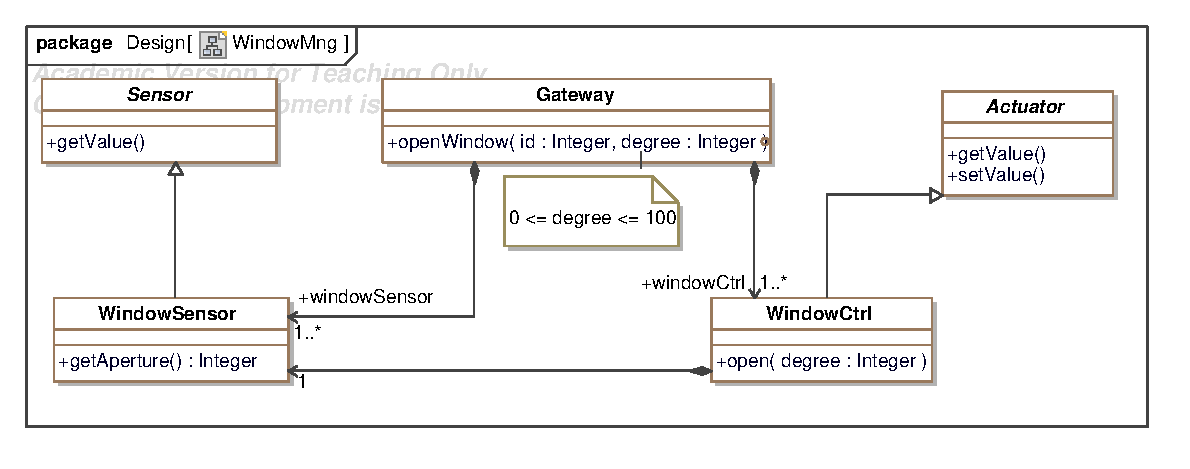
\includegraphics[width=.65\linewidth]{domainEngineering/Images/WindowMngDesign.eps} \\
 \caption{Dise�o de la caracter�stica \emph{WindowMng}.}
 \label{domain:fig:designWindowMng}
\end{figure}

las interfaces gr�ficas de usuario y de simulaci�n se extienden de un modo similar al de la iteraci�n anterior. La Figura~\ref{domain:fig:GUIWindowMng} muestra el aspecto visual de dichas interfaces.

%%=============================================================================================================%%
%% NOTA(Pablo): Todo esto se puede suprimir                                                                    %%
%%=============================================================================================================%%
%%
%% Para el caso de las dos interfaces gr�ficas se ha seguido un proceso similar que el utilizado en la
%% caracter�stica \emph{HeaterMng}, es decir, volviendo a definir las clases parciales que implementan a las
%% interfaces gr�ficas se a�aden nuevos controles del tipo pesta�a. De este modo las interfaces muestran un
%% dise�o como el representado en la figura \ref{domain:fig:GUIWindowMng}, en la cual en la parte superior de
%% la izquierda se ilustra la interfaz gr�fica del Gateway con la pesta�a global que controla todas las
%% ventanas, mientras que en la parte superior de la derecha se ilustra el dise�o destinado a controlar una
%% ventana espec�fica. En la parte inferior de la figura se muestra la interfaz gr�fica para el simulador.
%%
%%=============================================================================================================%%

%%=============================================================================================================%%
%% HECHO(Pablo): Quita una interfaz gr�fica para el control de ventanas e intenta que las dos te queden en una  %%
%%              misma l�nea                                                                                    %%     %%=============================================================================================================%%
\begin{figure}[!tb]
 \centering
 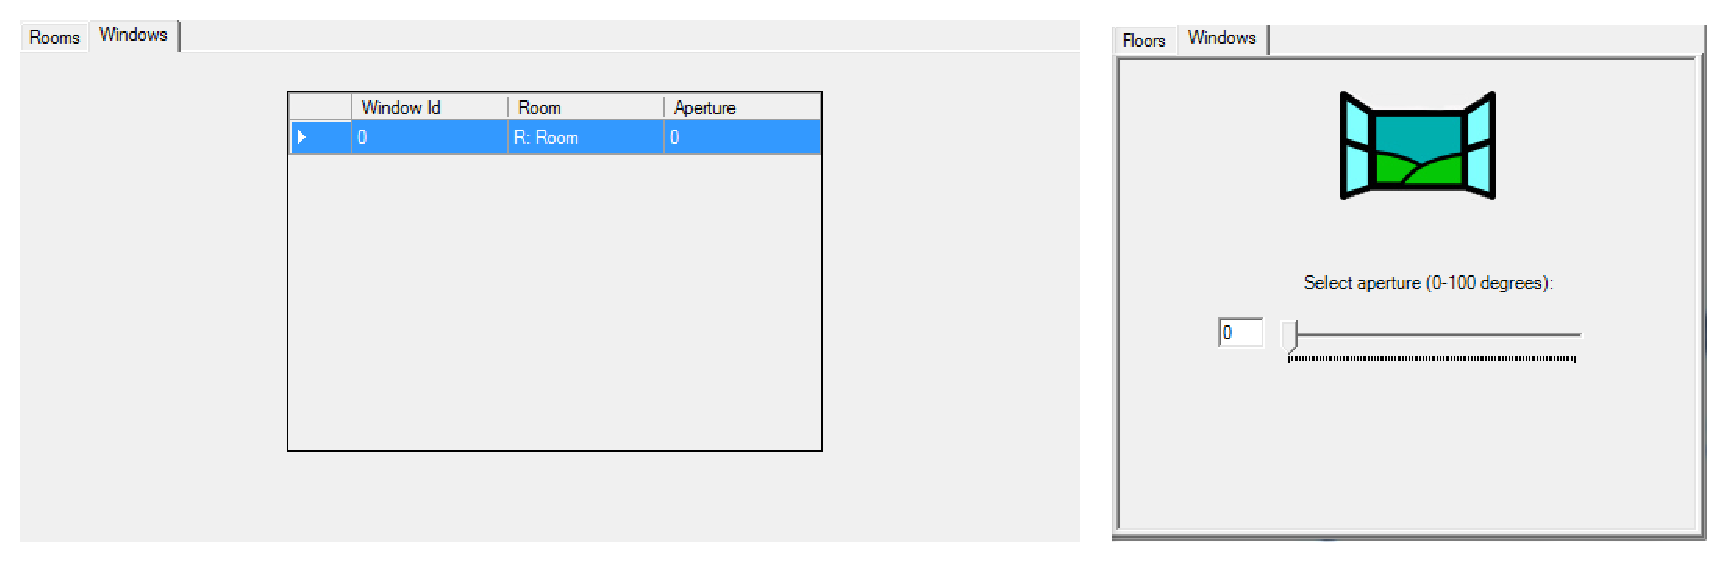
\includegraphics[width=.70\linewidth]{domainEngineering/Images/GUIWindowMng.eps} \\
 \caption{Dise�o de las interfaces gr�ficas para la caracter�stia \emph{WindowMng}}
 \label{domain:fig:GUIWindowMng}
\end{figure}

Al igual que en la iteraci�n anterior, una vez implementada la caracter�stica, se realizan una serie de pruebas para comprobar la correcci�n de la implementaci�n.

%%=============================================================================================================%%
%% NOTA(Pablo): Todo esto se puede suprimir                                                                    %%
%%=============================================================================================================%%
%%
%% Para las pruebas en esta caracter�stica se han realizado una serie de test, que han seguido el siguiente
%% procedimiento:
%%
%% \begin{enumerate}
%% \item Se han creado una serie de instancias del hogar inteligente con diferente n�mero de ventanas
%%         repartidas por distintas habitaciones.
%% \item Por cada instancia se realizan los siguientes casos de prueba:
%%    \begin{enumerate}
%%        \item Se modifica la apertura de las todas las ventanas, a trav�s de la pesta�a de
%%              control global de la caracter�stica, en la interfaz gr�fica del Gateway, y se comprueba
%%              en el simulador y en el propio Gateway.
%%        \item Por cada ventana se modifica su apertura, de modo individual a trav�s de su pesta�a
%%              espec�fica.
%%    \end{enumerate}
%% \end{enumerate}
%%
%%=============================================================================================================%%

La siguiente secci�n describe el proceso de desarrollo de la caracter�stica \emph{SmartEnergyMng}, la cual resulta d especial inter�s al tener que combinar de la forma adecuada la caracter�stica desarrollada en la secci�n actual con  la caracter�stica desarrolla en la secci�n anterior. 

\section{Iteraci�n 4: Control Inteligente de Energ�a}
\label{sec:domain:smartEnergy}
%%==================================================================%%
%% Author : P�rez Ruiz, Alejandro                                   %%
%% Author : S�nchez Barreiro, Pablo                                 %%
%% Version: 1.1, 18/06/2011                                         %%
%%                                                                  %%
%% Memoria del Proyecto Fin de Carrera                              %%
%% Domain Engineering/smartEnergy                                   %%
%%==================================================================%%

La caracter�stica para el control de inteligente de
la energ�a (\emph{SmartEnergyMng}) tiene dos objetivos principales:

\begin{enumerate}
	\item Siempre que los aparatos de control de la temperatura est�n
		  encendidos se deben cerrar todas las ventanas para evitar p�rdidas de energ�a.
	\item Almacenar los horarios de los habitantes de la casa, de modo que:
		\begin{itemize}
			\item Siempre que la casa est� vac�a los aparatos de control de la temperatura
					est�n apagados.
			\item Encender dichos aparatos con la suficiente antelaci�n para poder restablecer la temperatura elegida por el usuario a su regreso a casa.
		\end{itemize}
\end{enumerate}

Para realizar dicha funcionalidad, esta caracter�stica precisa usar las caracter�sticas de control autom�tico de ventanas (\emph{WindowMng}) y de la gesti�n de la temperatura (\emph{HeaterMng}).

\begin{figure}[!h]
 \centering
 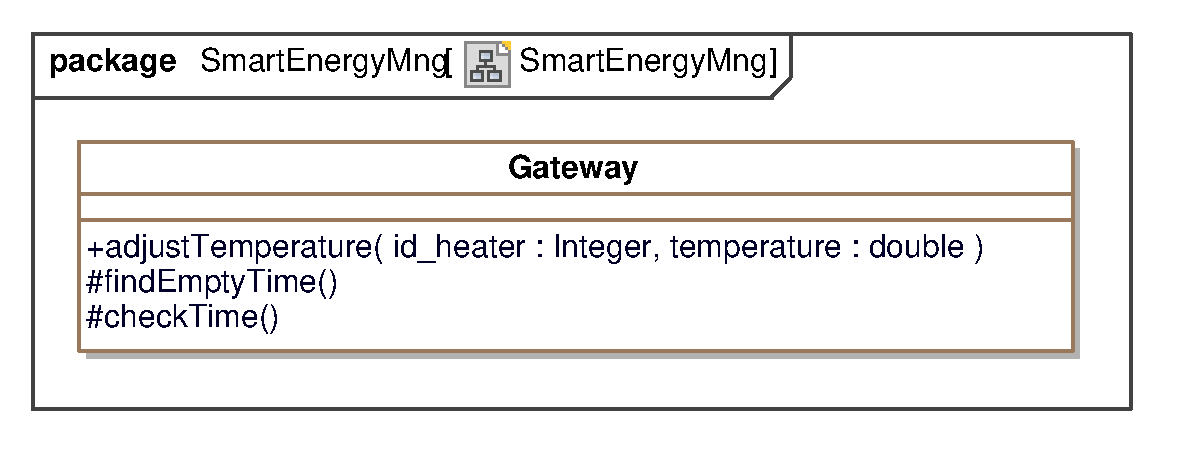
\includegraphics[width=.55\linewidth]{domainEngineering/Images/SmartEnergyMngDesign.eps} \\
 \caption{Dise�o del control inteligente de energ�a}
 \label{domain:fig:smartDesign}
\end{figure}

La Figura~\ref{domain:fig:smartDesign} muestra el dise�o de esta caracter�stica. Al igual que en las dem�s caracter�sticas hasta ahora descritas, la clase \imp{Gateway} se declara como parcial para a�adir nuevos m�todos, y en este caso, sobreescribir algunos de los ya existentes gracias al esquema presentado en la Secci�n~\ref{domain:sec:pattern}.


Los diferentes horarios de los habitantes de la casa se almacenan en una hoja XML~\cite{rusty:2004}. El objetivo de los m�todos \imp{findEmptyTime} es analizar las franjas de tiempo en las cuales la casa est� vac�a. El m�todo \imp{checkTime} se encarga, a intervalos regulares de tiempo, de conectar o desconectar los aparatos de control de la temperatura seg�n la casa est� vac�a, esperando la llegada de un habitante, u ocupada.

A la hora de implementar el cierre de las ventanas cuando los calefactores est�n funcionando, necesitaremos sobreescribir el m�todo \imp{adjustTemperature} de la versi�n del \imp{Gateway} para la caracter�stica de gesti�n de la temperatura (ver Figura~\ref{domain:fig:heaterMngDesign}). Para ellos usamos el patr�n descrito en la
Secci�n~\ref{domain:sec:pattern}. La implementaci�n del m�todo \imp{adustTemperature} se muestra en la Figura~\ref{domain:fig:codSmartEnergy}.

%%=======================================================================================================%%
%% HECHO(Pablo): Poner aqu� abreviado el m�todo adjustTemperature de la clase Gateway de la               %%
%%              caracter�stica SmartEnergy                                                               %%
%%=======================================================================================================%%
 \begin{figure}[ht!]
 \begin{center}
 \begin{footnotesize}
 \begin{verbatim}
 00 public void heaterAdjustTemperature(int id_heater, double temperature)
 01 {
 02      smartEnergyMng_heaterAdjustTemperature(id_heater, temperature);
 03 }
 \end{verbatim}
 \end{footnotesize}
 \end{center}
 \caption{Implementaci�n del m�todo heaterAdjustTemperature
          cuando la caracter�stica \emph{SmartEnergyMng} est� seleccionada}
 \label{domain:fig:codSmartEnergy}
 \end{figure}



%%=======================================================================================================%%
%% NOTA(Pablo): Esto ahora se borra                                                                      %%
%%=======================================================================================================%%
% la figura \ref{domain:fig:codSmartEnergy} cuando la caracter�stica actual est� seleccionada en una configuraci�n.
%

De nuevo se necesita definir las interfaces gr�ficas para esta caracter�stica. Para el caso de la interfaz de usuario, �nicamente se a�ade una nueva pesta�a global que contendr� un bot�n para activar o desactivar el control inteligente de energ�a, as� como especificar la temperatura que se desea tener cuando se reconecten los calefactores despu�s de que la casa haya estado vac�a. La interfaz gr�fica del simulador implementa una nueva pesta�a para esta caracter�stica. En dicha pesta�a se puede modificar el tiempo del sistema, con objeto de simular su paso. Adem�s,  se muestra una lista con los intervalos de tiempo en la que la casa se encuentra vac�a. (Ver Figura~\ref{domain:fig:SimulatorSmartEnergyMng}).

\begin{figure}[!tb]
 \centering
 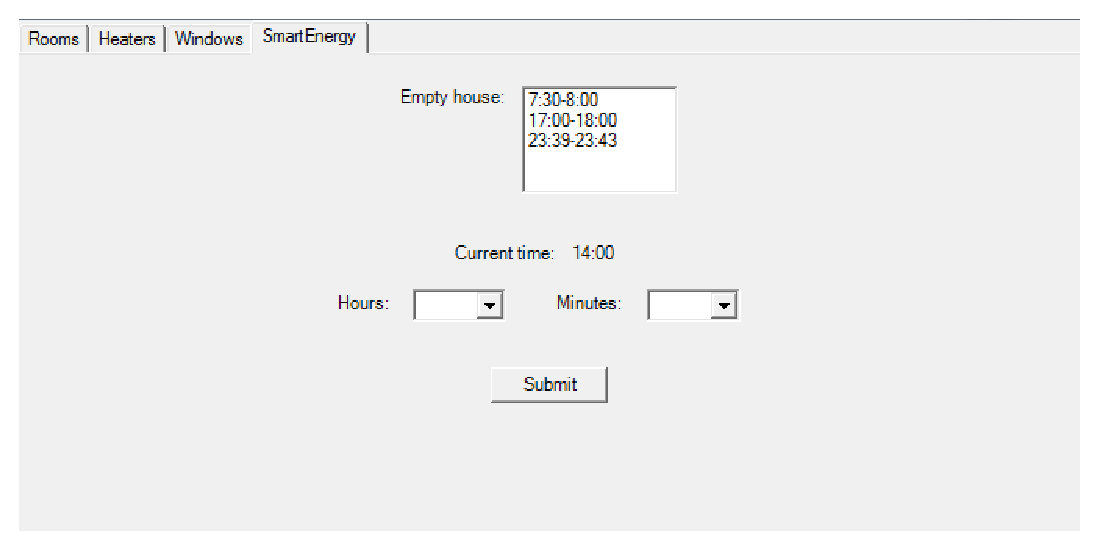
\includegraphics[width=.75\linewidth]{domainEngineering/Images/simulatorGUISmartEnergyMng.eps} \\
 \caption{Dise�o de la interfaz gr�fica de usuario para el simulador en la caracter�stica de \emph{SmartEnergyMng}}
 \label{domain:fig:SimulatorSmartEnergyMng}
\end{figure}

Las pruebas correspondientes a esta caracter�stica se han dividido en varios tests. El primer test debe verificar los m�todos destinados a procesar la hoja XML  con los horarios de los habitantes. Para ello se han probado diversos ficheros, conteniendo horarios con diferentes caracter�sticas, tales como situaciones en las cuales la casa nunca se encuentre vac�a.

El siguiente conjunto de tests est�n destinados a comprobar que los aparatos de control de la temperatura se apagan y se encienden correctamente de forma autom�tica cuando la casa est� vac�a. Para ellos se crean diferentes instancias de la casa con un n�mero arbitrario de dispositivos de control de la temperatura y se verifica que su comportamiento es el deseado.

La �ltima bater�a de tests se encarga de comprobar que las ventanas se cierran si el control inteligente de energ�a est� encendido y alguno de los aparatos de control de la temperatura entra en funcionamiento. Al igual que antes, se crean diferentes instancias de la casa y se comprueba su correcto funcionamiento.




\section{Otras iteraciones}

Como se ha podido observar en las iteraciones anteriores se sigue un procedimiento muy similar, por lo que no se proceder�n a describir por motivos de espacio y de no aburrir al lector.

% En UML las caracter�sticas son agrupadas como paquetes. Un \emph{paquete} es definido en UML como un elemento de modelado usado para agrupar otros elementos de modelado, para de este modo obtener un espacio de nombres para los elementos agrupados.
%La relaci�n \emph{merge} entre dos paquetes, indica que el contenido de ambos debe ser combinado, la especificaci�n UML establece que esta relaci�n se debe usar cuando los elementos de los paquetes tienen el mismo nombre y representan el mismo concepto\cite{omg:uml:2005}. Por lo que podemos definir un diagrama de paquetes como el mostrado en la figura \ref{domain:fig:packageDiagram}, en el que todas las caracter�sticas se conectan a trav�s de una relaci�n \emph{merge}. Por lo tanto, a trav�s de la figura \ref{domain:fig:packageDiagram} se puede reflejar que todas las caracter�sticas realizan una combinaci�n de sus elementos con el mismo nombre haciendo uso de las clases parciales.
%\begin{figure}[!tb]
% \centering
% 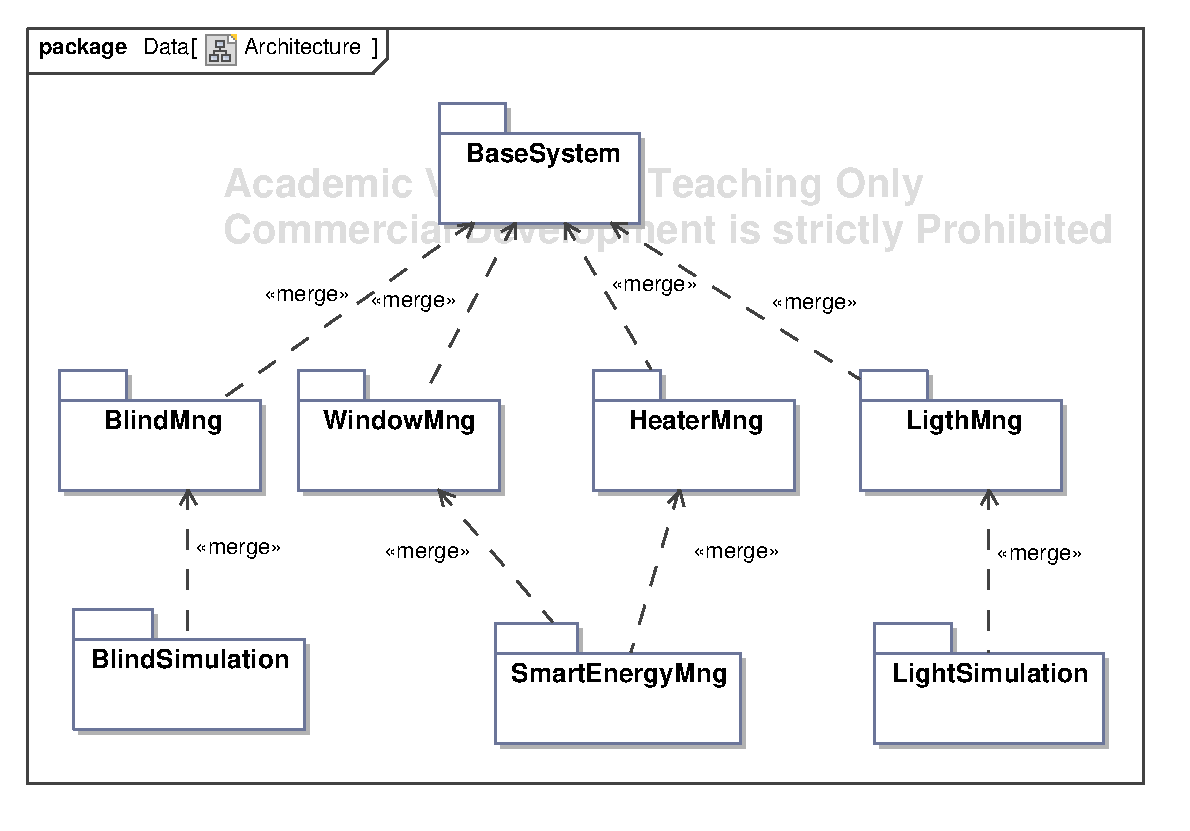
\includegraphics[width=.75\linewidth]{domainEngineering/Images/packageDiagram.eps} \\
% \caption{Diagrama de paquetes con todas las caracter�sticas.}
% \label{domain:fig:packageDiagram}
%\end{figure}

Tras realizar todas las iteraciones necesarias para implementar la ingenier�a de dominio, se consigue tener un sistema dividido que encapsula caracter�sticas que pueden ser combinadas y compiladas de diferentes maneras, siempre y cuando se respeten las restricciones b�sicas.

\section{Sumario}

En este cap�tulo se ha mostrado el proceso llevado a cabo para realizar la fase de ingenier�a de dominio en esta l�nea de productos software, en la cual se han utilizado las clases parciales de C\# como principal mecanismo para encapsular las caracter�sticas. No obstante, las clases parciales presentan alguna limitaci�n para encapsular correctamente, por lo que se han desarrollado y expuesto mecanismos para suplir estas limitaciones.

El siguiente cap�tulo mostrar� como utilizando la infraestructura desarrollada anteriormente, se pueden crear aplicaciones espec�ficas adaptadas a los requerimientos de los usuarios. 